\documentclass[11pt,fleqn,twoside]{article}
\usepackage{makeidx}
\makeindex
\usepackage{palatino} %or {times} etc
\usepackage{plain} %bibliography style 
\usepackage{amsmath} %math fonts - just in case
\usepackage{amsfonts} %math fonts
\usepackage{amssymb} %math fonts
\usepackage{lastpage} %for footer page numbers
\usepackage{fancyhdr} %header and footer package
\usepackage{mmpv2} 
\usepackage{url}
\usepackage{graphicx}

% the following packages are used for citations - You only need to include one. 
%
% Use the cite package if you are using the numeric style (e.g. IEEEannot). 
% Use the natbib package if you are using the author-date style (e.g. authordate2annot). 
% Only use one of these and comment out the other one. 
\usepackage{cite}
%\usepackage{natbib}

\begin{document}

\name{Andrew Tindall}
\userid{ajt7}
\projecttitle{Image Processing in the National Plant Phenomics Centre}
\projecttitlememoir{Image Processing in the National Plant Phenomics Centre} %same as the project title or abridged version for page header
\reporttitle{Progress Report}
\version{1.0}
\docstatus{Release Candidate}
\degreeschemecode{GG4R}
\degreeschemename{Computer Science \& Artificial Intelligence}
\modulecode{CS39440}
\supervisor{Hannah Dee} % e.g. Neil Taylor
\supervisorid{hmd1}
\wordcount{2773}

%optional - comment out next line to use current date for the document
%\documentdate{26th October 2011} 
\mmp

\setcounter{tocdepth}{3} %set required number of level in table of contents
\tableofcontents

\newpage

%==============================================================================
\section{Project Summary}
%==============================================================================
\subsection{Phenomics}
Before explaining the project, it is first important to understand the field in which it operates - namely that of plant phenomics.

Phenomics is a field of research in biology related to the systematic observation and analysis of ``phenomes", or biochemical and physical trait expression; and how their expression changes in result to environmental and genetic factors.

Phenomics is considered a rapidly emerging transdiscipline, requiring expertise in fields including ``genetics, molecular biology, cell biology, systems biology, and higher levels of phenotypic expression" alongside wider understanding of mathematical modelling and information sciences. \cite{Bilder200930}

The discipline has applications across many fields including public health \cite{Bilder200930} ; human genetics; biofuels; global food security \cite{Furbank2011635} ; and others due to its ability to allow understanding of how factors can affect traits, allowing for more development of more resilient crops, and predispositions to disease.

Plant Phenomics is a specific subset of phenomics, and concerns itself with ``the study of plant growth, performance and composition" \cite{Furbank2011635}, and is the subset observed in this project.

\subsection{Plant Phenomics and Food Security}
Food security is defined by the World Food Summit as a circumstance by which ``all people, at all times, have physical and economic access to sufficient, safe and nutritious food to meet their dietary needs and food preferences for an active and healthy life" \cite{WFS1996}.
This is increasing taken within the context of climate change, globalisation and corporatism, international relations, and the global economy, all of which impact on the ability to provide food through links at each stage of the supply change. With environments changing and often becoming less hospitable to life, there is a turn towards breeding high-yield crops which are resilient and adapted to future climates \cite{Furbank2011635}.

With traditional breeding no longer resulting in yield increases that can meet projected demand of staple crops\cite{Furbank2011635}, there is a need to turn to phenomics, which offers the ability to rapidly analyse large plant populations and thereby develop germplasm stocks that can meet current and future needs.

\subsection{Use of Image Processing in Phenomics}
Traditionally, methods for phenome observation would involve destructive techniques that remove entire plants or parts, and this results in the need for larger physical space and longer time periods for research. \cite{DeVylder01112012}

In recent years there has been a large focus on the development of high-throughput and non-destructive techniques, particularly in the analysis of Arabidopsis - a small flowering plant including Thale Cress which is used as a model organism due to being the first plant to have its genome sequenced in its entirety\cite{AGI2000}. Principle among this area is the use of image processing and analysis, which allows for remote screening of multiple traits with minimum disruption to specimens. \cite{DeVylder01112012}

LemnaTec are one of the eminent organisations involved in the field of plant phenomics, supporting research institutes around the world through provision of hardware and algorithms. This includes infrastructure at the recently developed National Plant Phenomics Centre (NPPC) at Aberystwyth University which utilises robotic plant handling and automated image capture and analysis to conduct phenomics on entire plant populations in the hopes of identifying plants with increased tolerance to adverse conditions \cite{IBERSnppc}; the work of which provides the basis for this project.

\subsection{Project Details}
This project seeks to develop a system capable of using multiple algorithms for the processing and analysis of automated image data sets of arabidopsis populations grown in a controlled environment in order to provide phenotype information and analysis about the plants. In doing so, it shall be comparable to, and build upon the  the work of the NPPC, and Rosette Tracker \cite{DeVylder01112012}.

The work has several limitations arising from multiple factors. Foremost is that of data collection. That the project requires the growth of populations of plants introduces inherent time factors into the project, which means datasets are time-limited, and this can hinder early analysis and testing of software. Additionally, variations in the environment for growth, and in terms of imaging, can present discrepancies in the data set, or even render parts of the set unviable for inclusion, such as due to an image being overexposed, or a camera being out of position for several frames of the set. Limitations also exist in terms of what can be achieved through visible-spectrum imaging, which is the broad focus of the project, as not everything can be observed at the scales and spectrum being used; however it may be possible for the project to utilise further imaging techniques such as IR imaging later into the project subject to the provision of data from the NPPC.

Ultimately, the finished work should output data that provides answers to important questions such as ``to what extent does the ede1 mutation affect growth rates and patterns?" and flowering times between different populations. The project may be judged a success should be it capable of providing the prerequisite steps and analysis to reach this stage, as well as data that allows conclusions about phenotypes to be made on these questions and others.



%==============================================================================
\section{Current Progress}
%==============================================================================
\subsection{Technologies and libraries}
There exists numerous libraries for image processing and analysis, including ImageJ and OpenCV. Each of these tends to implement common processing techniques such as Canny and Sobel Edge Detection, image segmentation, etc.

ImageJ is a public domain image processing and analysis tool written for the java programming language. OpenCV is a similar, open source implementation for C++, C and Python and has over 2500 optimised algorithms \cite{opencv}. Wrappers exists for OpenCV, including JavaCV, which allows for its use in java.

Both are common in academic environments, although OpenCV appears to enjoy wider uptake across sectors, perhaps due to being available across multiple programming languages, and comprehensive documentation for the C++ implementation.

After preliminary reading and research into the kind of techniques required to undertake this project, and after consideration of familiarity with each library, and the required programming languages for such; it was decided that initial prototyping would make use of JavaCV to provide the underlying functionality of the project. Whilst additional methods and algorithms will likely be required to written regardless of library, it is possible that should issues with JavaCV arise in any systematic or seriously hindering way, use of switching to other libraries shall be considered prior to formalisation of a stable code branch.

\subsection{Language selection}
Java was selected as the programming language for the implementation of  this project due to two primary reasons. Firstly, it is the language in which the most experience is currently held, and so work can focus on actual implementation rather than learning the language itself. Secondly, Java is capable of running on the majority of platforms and hardware configurations without any notable or significant differences in each instance.

Subjection to the completion of all planned features, and excluding any earlier switches due to any arising issues that render the current language and libraries unusable for the project, it shall be explored the possibility of porting the project to other languages as part of the refactoring process - for example Ruby, with which some familiarity is held, or Python or C++ which are commonly used for the development of image processing and analysis systems.

In doing this, it should be achievable to decrease computation times that result from the java runtime environment�s resource consumption, and allows for greater understanding of core concepts and furtherment of knowledge of programming languages with which current knowledge is lesser compared to java. 

Any such decisions on language or library porting shall be done on the basis of maintaining a stable branch in its then-current state so that a functioning system may be delivered regardless of any issues occurring in these forks. 

Should any forks be completed, they shall be evaluated and possibly replace the stable branch for submission, or if entirely equivalent, both be submitted as viable code bases.

\subsection{System Overview}
Before any prototyping was begun, it was reviewed at a top-down level what features the project would require. Broadly, the system can be broken down into three categories: Image Collection, Image Processing, and Image Analysis.

Each of these stages were further broken down until individual processes were defined, and this was used as the basis for prototyping and development, by working chronologically through the processes, amending and introducing new processes where needed or beneficial.

\begin{figure}[system-overview]
\centering
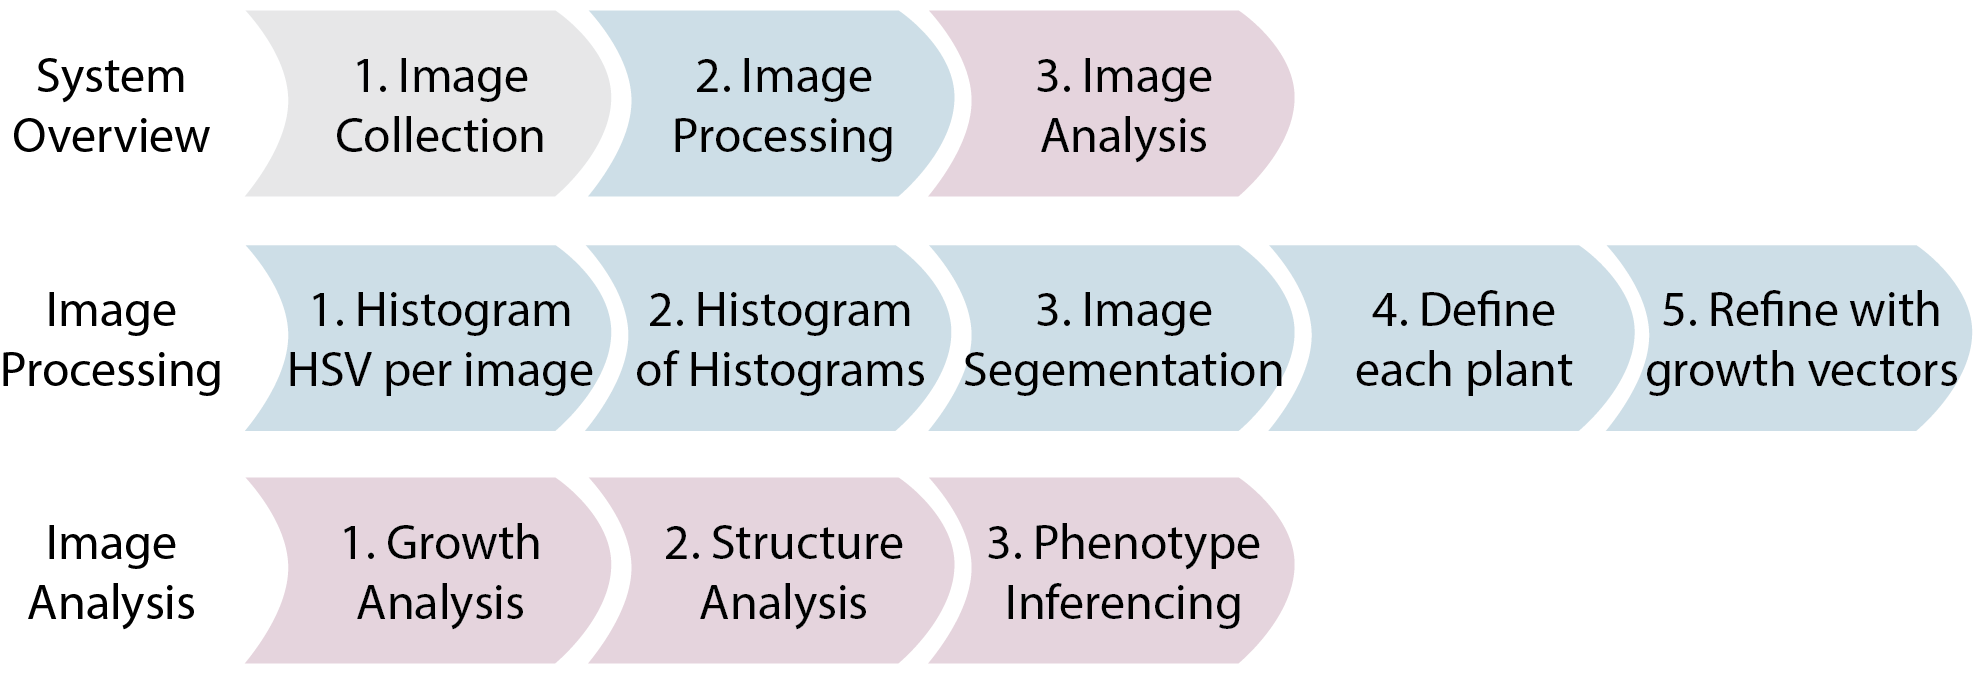
\includegraphics[width=0.85\textwidth]{system-overview.png}
\caption{Breakdown of system processes including image processing and analysis.}
\label{fig:system-overview}
\end{figure}

As a result of this methodology, the current system overview is as displayed in figure 1, and although likely to remain broadly the same, sections are likely to be added, removed, or otherwise adjusted as the project progresses.

\subsection{Prototyping and Experimentation}
The project is being developed incrementally, with prototypes of each feature being developed and refined before moving onto the next feature. Eventually these refined prototypes will be revised and merged into a stable code branch, with additional prototyping forks being merged in at later dates.

The first code developed was for handling image input and output, and under OpenCV/JavaCV, is mere lines long. This code forms the basis of all following features, as the vast majority of work requires access to the raw data set or processed images.

The next feature to be developed was a rudimentary image segmentation method, which initially took a pre-defined hue, and matched this against the HSV colour space for a given image, returning a segmented image showing just pixels of that hue. Figure 2 shows the result of this code run against a test image.

\begin{figure}[seg-test]
\centering
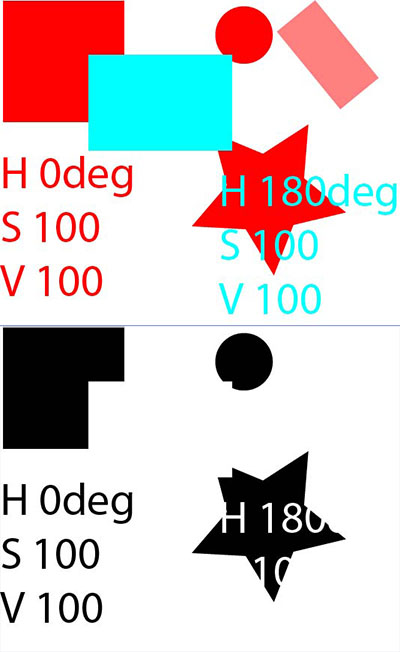
\includegraphics[width=0.3\textwidth]{seg-test-compare.jpg}
\caption{Comparison of test image input with results of preliminary image segmentation}
\label{fig:seg-test}
\end{figure}

Following the successful test, the segmentation method was adapted to make use of histogram information, as real life objects are not just a single hue, and so to adequately detect them, we must look at multiple values across specific ranges. Segmentation at this stage would only highlight the most common hue value �bucket�, which in images from earlier in the dataset, would not correspond to the plants; and depending on the fuzziness of each bucket, would effectively just create a black and white version of the original image.

\begin{figure}[seg-histo]
\centering
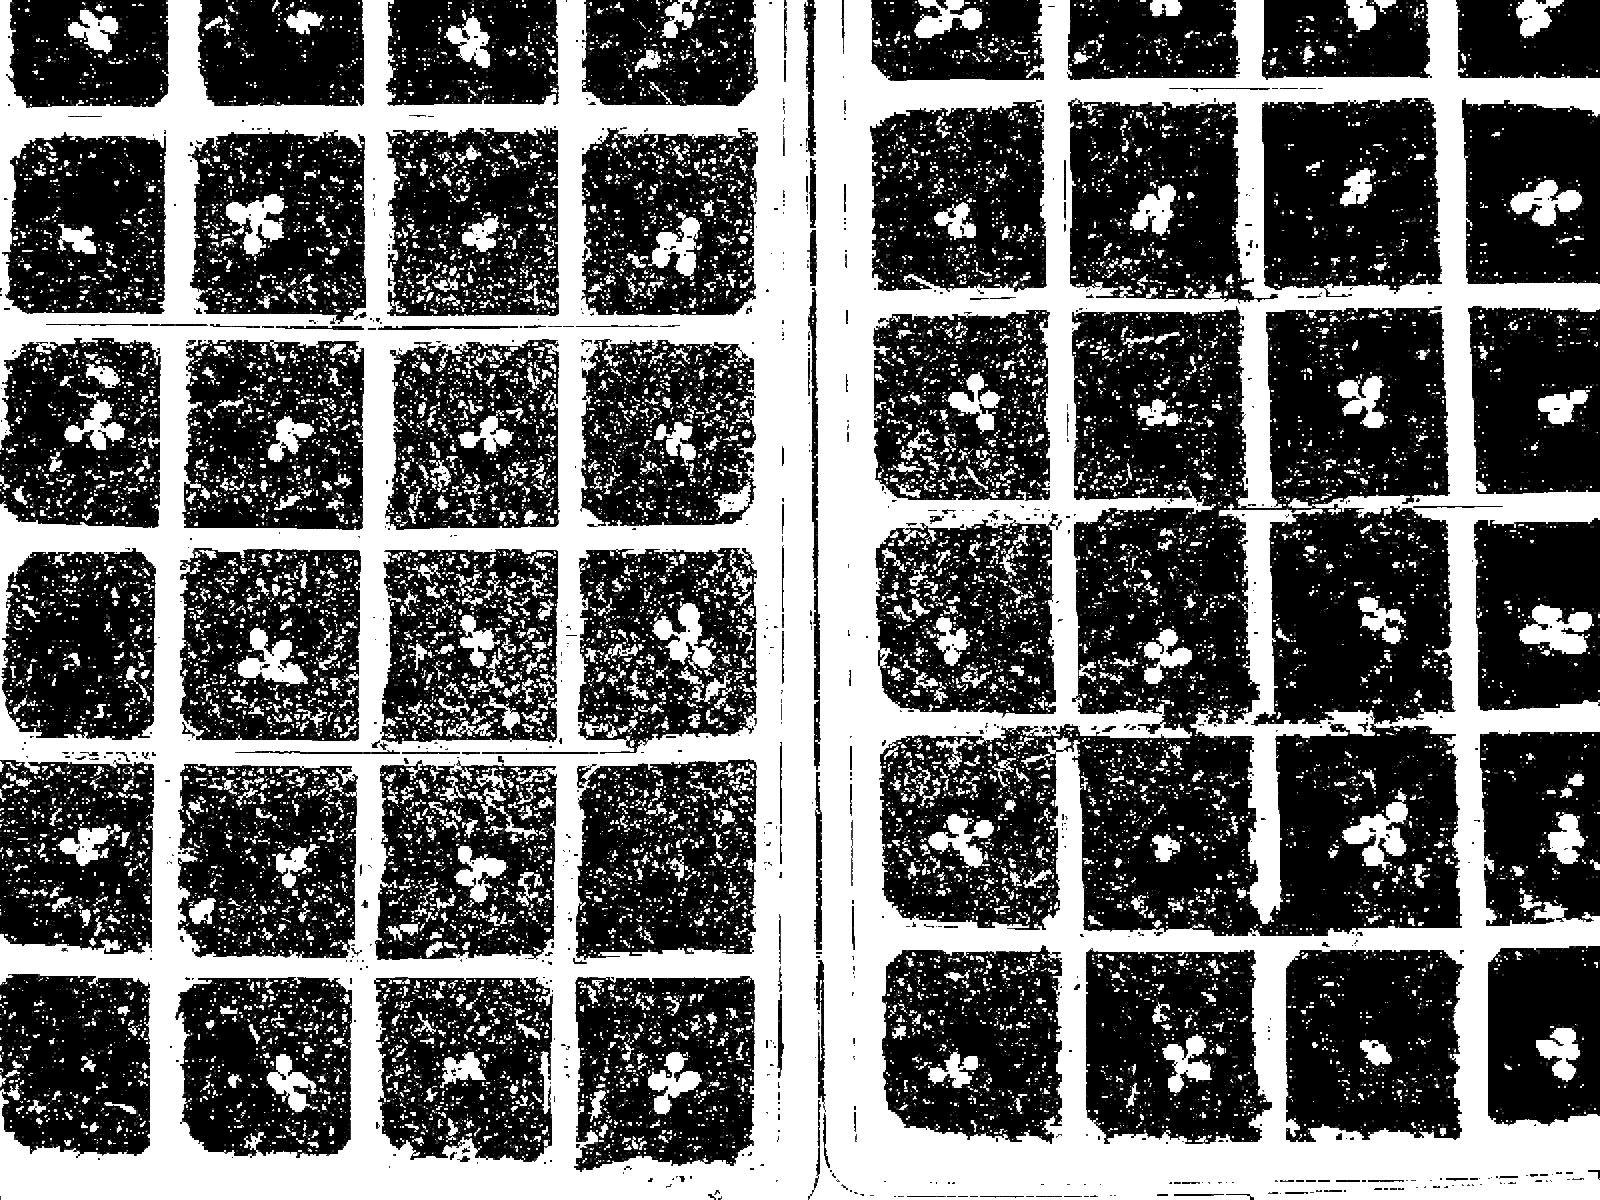
\includegraphics[width=0.3\textwidth]{seg-histo.jpg}
\caption{Naive histogram-derived image segmentation}
\label{fig:seg-histo}
\end{figure}

It was decided that a solution to the issues that presented when using histograms to define segmentation, was to use histograms across the entire data set as a form of �voting� for the hue ranges to segmentate on the current image in the set. This would thereby allow images later in the set, which would in most cases contain an increasing amount of plant-specific colours inherent due to the growth of plants meaning they cover more of an image, have an influence over the dominant colours that define a plant. This solution is not yet fully implemented however is projected for completion by the end of week 47, 2012.

As per the system overview, the next feature to be prototyped shall be that of plant detection, including defining boundaries for each plant, potentially through use of environmental features, as well as plant diameter and compactness as used in Rosette Tracker \cite{DeVylder01112012}.


%==============================================================================
\section{Planning}
%==============================================================================
\subsection{Methodology}
In undertaking this project, it was explored what development methodologies could be applied, such as the waterfall model,  rapid application development, or iterative and incremental design.

Under the waterfall model, the project is completed in seven phases which are followed in order: requirements specification; design; implementation; integration; testing; installation; and maintenance. In this way, all requirements and concepts are laid out in detail before any implementation begins. This can create issues where it is not clear the exact route to be taken to complete the tasks at hand, or serious difficulties arise preventing implementation of a section; and if requirements change, potentially large sums of work can be invalidated.

With rapid application development (rad), a project consists of just four phases: Requirements planning, where the requirements, scope, and constraints are defined; user design, where prototyping is used to understand and modify the specification to fit the needs of the task; construction, where the application is developed; and cutover, where testing and delivery take place. This allows for a far more flexible approach than under waterfall, with input and changes welcomed at each stage, whilst still maintaining a design-first approach.

In Iterative and Incremental Design, there are four phases, which may iterate numerous times. Inception is used to outline requirements and scope at a high level; elaboration then allows for the drawing up of a more defined working structure; this is then incrementally produced in the construction phase, after which the system is transitioned into the operating environment. Through the use of iteration, the project can evolve over time beginning with simple implementation of parts of the structure, making use of previous iterations to expand and improve existing and future features.

It was decided that as the project was wide enough to provide uncertainty in low-level requirements, an iterative and incremental model would be most suitable, so as to provide for development of features in a modular form that could expand in scope as and when needed. 

In doing this, a working product can be derived from a broad system overview, or system control list, and each feature can be implemented easily and in a manageable and scheduled manner. This means a clear road-plan exists whilst also providing fluidity and adaptability in the project.

\subsection{Project Schedule}
Figure 4 depicts the current project road-plan through to the final deliverable of the final presentation, taking into account likely risks or delays caused by external factors such as exams starting in week 3, 2013; conference attendances throughout the same timeframe as the project, and temporary incapacity due to illness. 

Each task prior to Week 1, 2013, corresponds to development of key features through an iterative process, and this deadline is set to ensure a core set of features are delivered. Following weeks account for the formalisation and refactoring of this code base, whilst exploring other opportunities to build upon this core.
The plan provides a full six weeks where the code should be locked and work is focused entirely on delivery of the final report. This is reflective of the weighting of the report, as well as the need to ensure functional, documented code prior to the final delivery of the project.

Given the nature of iterative and incremental development, several weeks have been set aside for the exploration of techniques not yet specified in the control list / system overview.

By week 50, the code base should contain functionality for the core features required for basic analysis, namely colour frequency analysis, image segmentation, and plant classification. In the following weeks, additional algorithms are to be added to further refine these features, as well as to provide analysis in other areas, for example, leaf density.

In addition to the tasks listed, it is hoped that discussions shall be held with staff and researchers involved in the National Plant Phenomics Centre at IBERS; and it is likely that such talks will help shape the direction of the project, such as by providing insight into potential problems for the system to attempt to solve, or access to new datasets potentially using different imaging techniques. Changes due to this are already partially factored into the assigned time frames for the completion of each task.

\begin{figure}[gantt]
\centering
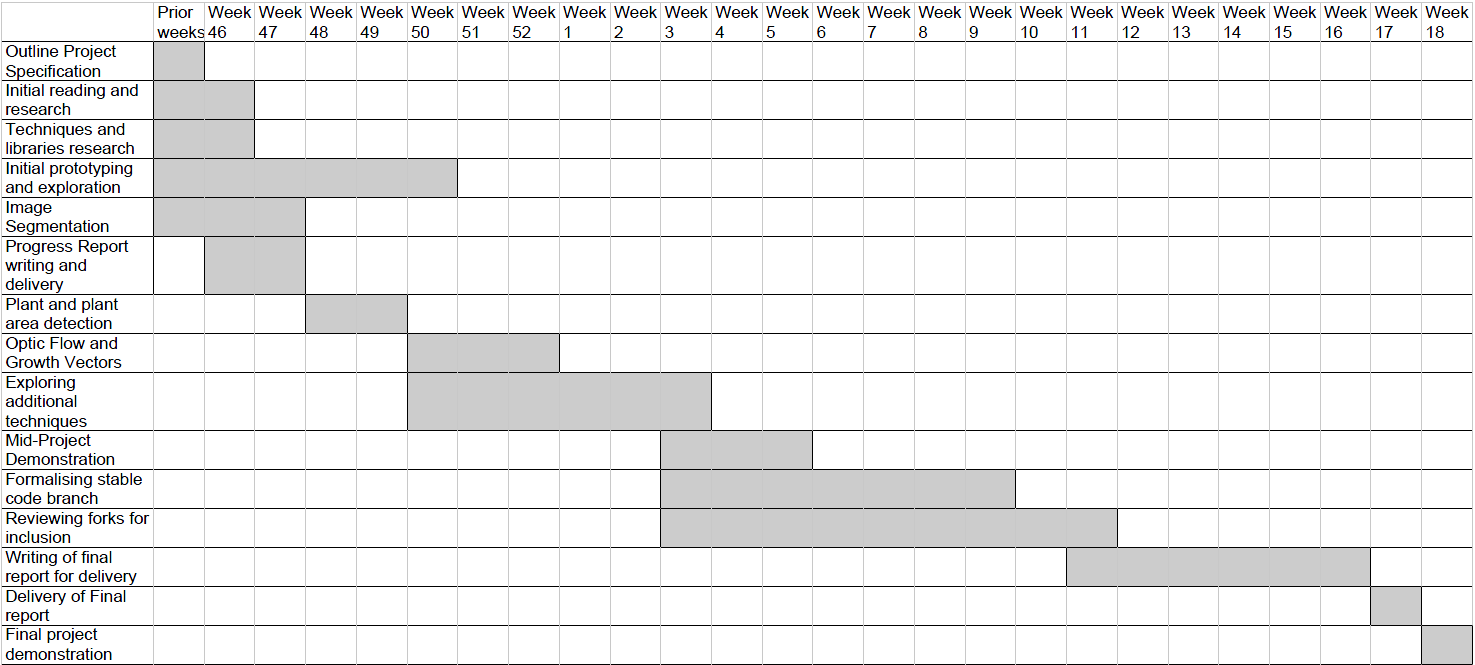
\includegraphics[width=1\textwidth]{gantt.png}
\caption{Gantt diagram showing project road-plan through to week 18, 2013 }
\label{fig:gantt}
\end{figure}

\subsection{Demonstrations}
Completion of the project includes two demonstrations of the system. Once during week 5, 2013, and again during week 18, 2013. In both instances, it is hoped that results of the analysis from implemented features can be presented, where possible demonstrating the processing and analysis live.

In the mid-project demonstration, it is to be expected that there would be less data to show due to not all analysis features being implemented at that stage, as well as the possibility of additional data sets being made available throughout the duration of the project, including after this demonstration. However, it should be considered sufficient to demonstrate, more than merely �proof of concept�, that the system is functional and capable of producing real phenomic information based on the provided input data, even if the output data is limited in its scope at this stage.

For the final demonstration, it is expected that more findings of project can be reported, namely at least some of the questions laid out in prior sections of this document. In addition, a live demonstration of the software, should also be conducted, as well as potential discussion of future scope for research and development from this project post-delivery.

With both demonstrations, access to a projector, and a device capable of running presentation software is a clear requirement. Ensuring the device is also capable of processing data in real-time and within the timeframe of the demonstration is also a major consideration, which may involve the selection of a subset of a data set or other such preparation to ensure execution times are permissible.







\nocite{*} % include everything from the bibliography, irrespective of whether it has been referenced.

% the following line is included so that the bibliography is also shown in the table of contents. There is the possibility that this is added to the previous page for the bibliography. To address this, a newline is added so that it appears on the first page for the bibliography. 
\newpage
\addcontentsline{toc}{section}{Annotated Bibliography} 

%
% example of including an annotated bibliography. The current style is an author date one. If you want to change, comment out the line and uncomment the subsequent line. You should also modify the packages included at the top (see the notes earlier in the file) and then trash your aux files and re-run. 
%\bibliographystyle{authordate2annot}
\bibliographystyle{IEEEannot}
\renewcommand{\refname}{Annotated Bibliography}  % if you put text into the final {} on this line, you will get an extra title, e.g. References. This isn't necessary for the outline project specification. 
\bibliography{mmp} % References file


\end{document}
